\documentclass[12pt]{article}

\input{physicsPream}

\begin{document}

%----------BEGIN TITLEPAGE----------

\begin{titlepage}

  \title{Lab 2: Diffraction}
  \author{\textbf{Ryan Wojtyla} \\
    Xzavier Flowers \\
    Joshua Newman \\
    Akshath Wikramanayake \\}
  \date{October 23, 2018}

  \maketitle

\begin{center}
  {\Large Abstract}
\end{center}

\qq In this lab, the effects of shining light through different types of slits
were observed. The resulting patterns were sketched and measured, then analyzed
using the diffraction equation for single slits, \(a = \frac{m \lambda D}{y}\),
and the interference equation for double slits, \(d = \frac{m \lambda
  D}{y}\). The error of all the measured quantities was propagated throughout
the calculations.

\thispagestyle{empty}

\end{titlepage}

%-----------END TITLEPAGE-----------

\section{Experiments}

%----------BEGIN EXPERIMENT 1----------

\subsection{Experiment 1: Diffraction from a Single Slit}

\subsubsection{Data}

\begin{figure}[H]
  \label{tab:1.1}
  \caption{\textbf{Table 1.1}: The data for the \SI{0.04}{\milli\meter} single
    slit.}
  \makebox[\textwidth][c]{
    \begin{tabular}{|>{\bfseries}c | c | c |}
      \hline
      & \textbf{\(m=1\) (\si{\centi\meter})} & \textbf{\(m=2\) (\si{\centi\meter})} \\
      \hline                                                 
      Distance between side orders     & 3.4 \(\pm\) 0.05 & 7.0 \(\pm\) 0.05 \\         
      Distance from center to side (y) & 1.7 \(\pm\) 0.025 & 3.5 \(\pm\) 0.025 \\
      Calculated slit width            & \num{3.81e-3} \(\pm\) \num{5.61e-5} &
                                                                           \num{3.71e-3}
                                                                           \(\pm\)
                                                                           \num{2.73e-5}
      \\
      \% difference                    & 4.87 \(\pm\) \num{0.101} & 7.52 \(\pm\)
                                                                    \num{0.0783} \\
      \hline
    \end{tabular}
  }
\end{figure}

\[\text{Slit-to-screen distance(}D\text{)} = 96 \pm 0.05 \si{\centi\meter}\]

\begin{figure}[H]
  \label{pic:exp1}
  \begin{center}
    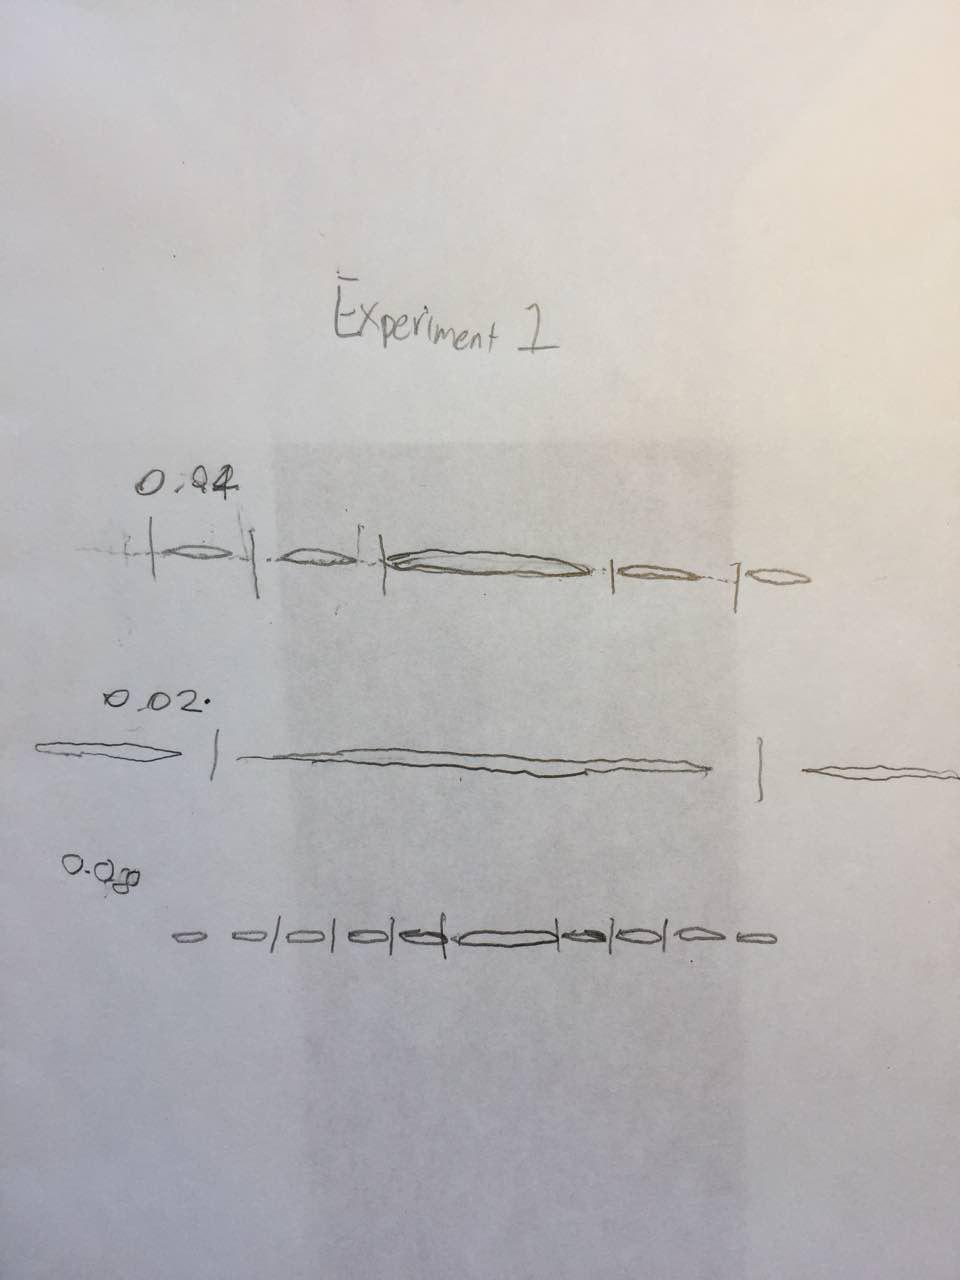
\includegraphics[scale=0.35]{exp1.jpg}
  \end{center}
  \caption{The sketches of the observed diffraction patterns. The top is of
    \SI{0.04}{\milli\meter}, the middle is of \SI{0.02}{\milli\meter}, and the
    bottom is of \SI{0.08}{\milli\meter}.}
\end{figure}

\subsubsection{Analysis}

\qq For the value of the slit-to-screen distance and the values measured for the
distance between the side orders, the error is \(\pm 0.05 \si{\centi\meter}\)
because that is half of the smallest increment of measurement on our measuring
device, a ruler. When the measured values for the distance between the side
orders are divided to find the distance from the center of the screen to the
side of the envelope (\(y\)), the error of the measured values must also be
divided by the same amount. Therefore, since the measured values are divided by
\(2\), the error must also be cut in half. The error for \(y\) is \(\pm 0.025
\si{\centi\meter}\).  

\qq The slit width, \(a\), is calculated with \(a = \frac{m \lambda D}{y}\),
where \(m \in \mathbb{Z}\) is the order number, \(\lambda\) is the wavelength, \(D\) is the
distance between the slit and the screen onto which the image is projected, and
\(y\) is the distance from the center of the screen to the side of the
\(m^{\text{th}}\) minimum. The average wavelength of the diode laser is
\SI{670}{\nano\meter}. For the first order, when \(m = 1\), the base value of
the slit width can be calculated:

\begin{align*}
  a &= \frac{m \lambda D}{y} \\
  a &= \frac{(1) (\num{670e-7}) (96)}{(1.7)} \\
  a &= \num{3.81e-3} \si{\centi\meter} \\
\end{align*}

Since the two values with uncertainty, \(D\) and \(y\), are being divided, the
error of \(a\) can be found with:

\begin{align*}
  \delta a &= a \sqrt{\left( \frac{\delta D}{D} \right) ^2 + \left( \frac{\delta
             y}{y} \right) ^2 } \\
  \delta a &= (\num{3.81e-3}) \sqrt{\left( \frac{(0.05)}{(96)} \right) ^2 +
             \left( \frac{(0.025)}{(1.7)} \right) ^2} \\
  \delta a &= \num{5.61e-5}\si{\centi\meter} \\
\end{align*}

The same method was used to find the slit width for the second order, where \(m
= 2\) and \(y = 3.5 \pm \num{0.025} \si{\centi\meter}\).

\qq The percent difference between the experimental values of the slit width,
\(a_{e1} = \num{3.81e-3} \pm \num{5.61e-5} \si{\centi\meter}\) and
\(a_{e2} = \num{3.71} \pm \num{2.73e-5} \si{\centi\meter}\) respectively, and
its theoretical value, \(a_t = \num{0.04} \si{\milli\meter}\), can be found with
\\\( \%_{diff} = \frac{\left| a_e - a_t \right|}{\left( \frac{a_e + a_t}{2} \right)} \cdot
100\% \). The percent difference for the first order is:

\begin{align*}
  \%_{diff} &= \frac{\left| a_{e1} - a_t \right|}{\left( \frac{a_{e1} + a_t}{2} 
              \right)} \cdot 100\% \\
  \%_{diff} &= \frac{\left| (\num{3.81e-5}) - (\num{0.04e-3}) \right|}{\left(
              \frac{(\num{3.81e-5}) + (\num{0.04e-3})}{2} \right)} \cdot 100\%
  \\
  \%_{diff} &= 4.87\% \\
\end{align*}

Since the only value with error in the calculation, \(a_{e1}\), is in both the
numerator and denominator, the error propagation equation from above,
\(\delta \%_{diff} = \%_{diff} \sqrt{\left( \frac{\delta x}{x} \right) ^2 +
  \left( \frac{\delta y}{y} \right) ^2 } \), can be used to find the error in
the percent difference of the first order:

\begin{align*}
  \delta \%_{diff} &= \%_{diff} \sqrt{\left( \frac{\delta a_{e1}}{a_{e1}}
                     \right) ^2 + \left( \frac{\delta a_{e1}}{a_{e1}} \right )
                     ^2} \\
  \delta \%_{diff} &= (4.87) \sqrt{\left(
                     \frac{(\num{5.61e-5})}{(\num{3.81e-3})} \right) ^2 +
                     \left( \frac{(\num{5.61e-5})}{(\num{3.81e-3})} \right) ^2}
  \\
  \delta \%_{diff} &= \num{0.101} \% \\
\end{align*}

These methods were also used to calculate the percent difference and its error for
the second order.

\subsubsection{Questions}

\subsubsubsection{}

\qq The distance between the minima decreases as the slit width increases.

%-----------END EXPERIMENT 1-----------

%----------BEGIN EXPERIMENT 2----------

\subsection{Experiment 2: Interference from a Double Slit}

\subsubsection{Data}

\begin{figure}[H]
  \label{tab:2.1}
  \caption{\textbf{Table 2.1}: The data for the
    \SI{0.04}{\milli\meter}/\SI{0.025}{\milli\meter} double slit.}
  \makebox[\textwidth][c]{
    \begin{tabular}{|>{\bfseries}c | c | c |}
      \hline
      & (\(m=1\)) (\si{\centi\meter}) & (\(m=2\)) (\si{\centi\meter}) \\
      \hline
      Distance between side orders         & 0.5 \(\pm\) 0.05 & 1.0 \(\pm\) 0.05 \\
      Distance from center to side (\(y\)) & 0.25 \(\pm\) 0.025 & 0.5 \(\pm\) 0.025 \\
      Calculated slit separation           & \num{2.57e-2} \(\pm\) \num{2.57e-3} & \num{2.57e-2}
                                                                                   \(\pm\)
                                                                                   \num{1.29e-3} \\
      \% difference                        & 2.76 \(\pm\) \num{0.390} & 2.76
                                                                        \(\pm\)
                                                                        \num{0.196} \\
      \hline
    \end{tabular}
  }
\end{figure}

\[\text{slit-to-screen distance (}D\text{)} = 97 \pm 0.05 \si{\centi\meter}\]

\begin{figure}[H]
  \label{pic:exp2}
  \begin{center}
    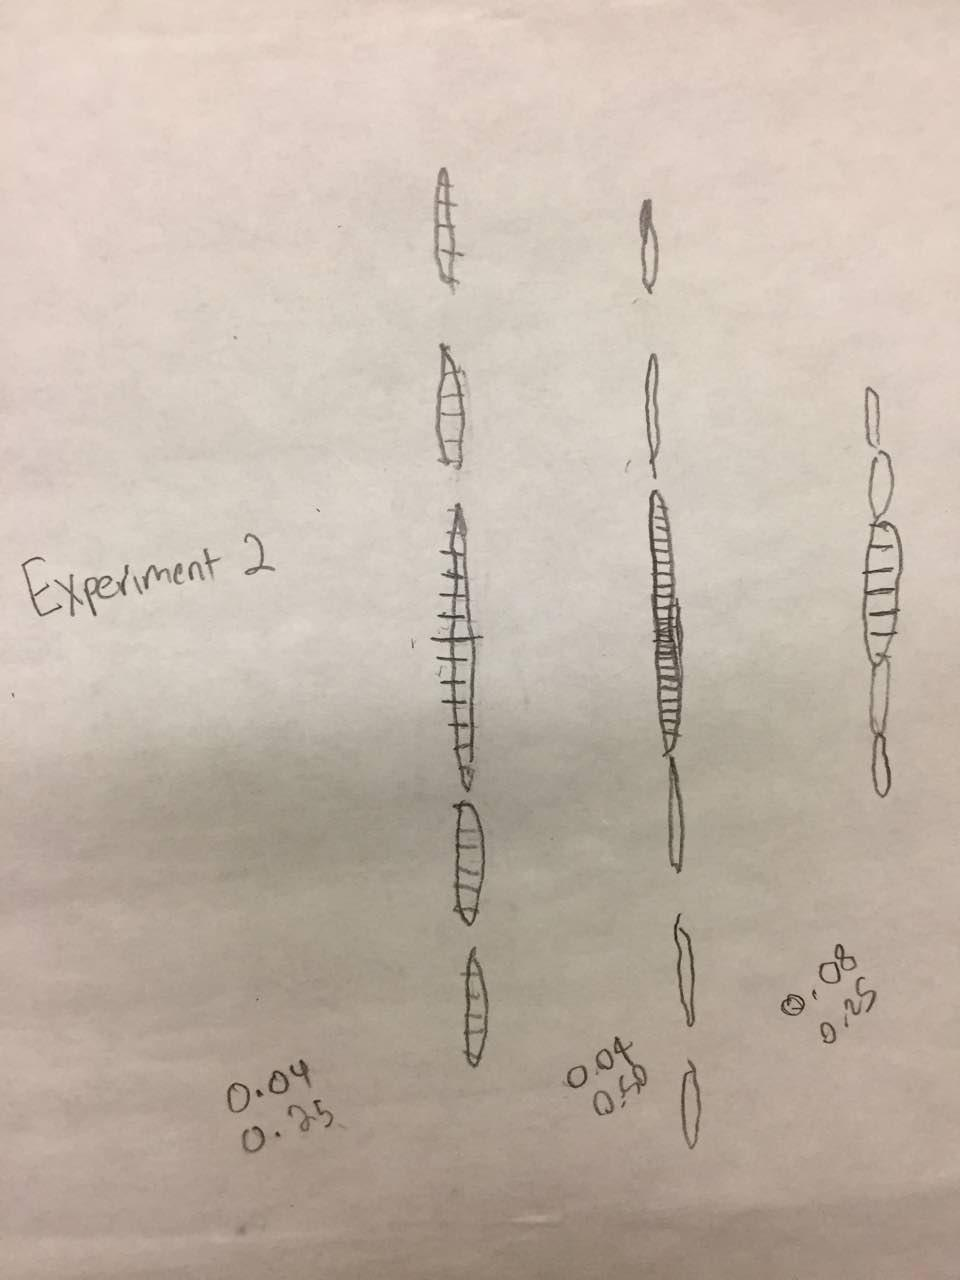
\includegraphics[scale=0.4]{exp2.jpg}
  \end{center}
  \caption{Sketches of the various interference patterns.}
\end{figure}

\subsubsection{Analysis}

\qq To get the values of \(y\) for the first and second orders, the measured
distance between the side orders was divided by a constant, \(2\). Since the
values were divided by a constant, the error of the original value must be
divided by that same constant, \(\delta y = \pm 0.025 \si{\centi\meter}\).

\qq The slit separation was calculated the same way as the slit width in
Experiment 1, using \(d = \frac{m \lambda D}{y}\), where \(m \in \mathbb{Z}\) is
the order, \(\lambda = \SI{670}{\nano\meter}\) is the average wavelength of the
diode laser, \(D = 97 \pm 0.05\si{\centi\meter}\) is the distance between the
slit and screen, and \(y_1 = 0.025 \pm 0.025 \si{\centi\meter}\) and
\(y_2 = 0.5 \pm 0.025 \si{\centi\meter}\) are, respectively, the distances from
the center of the pattern to the first and second order maxima. The error of the
slit separation was also calculated using the same formula from Experiment 1, 
\(\delta a = a \sqrt{\left( \frac{\delta D}{D} \right) ^2 + \left( \frac{\delta
y}{y} \right) ^2 } \).

\qq The percent difference between the experimental values of the slit
separation, \(a_{e1} = \num{2.57e-2} \pm \num{2.57e-3} \si{\centi\meter}\) and
\(a_{e2} = \num{2.57e-2} \pm \num{1.29e-3} \si{\centi\meter}\), and its
theoretical value, \(a_t = 0.25 \si{\milli\meter}\), may be determined the same
way as in Experiment 1, by using
\(\%_{diff} = \frac{\left| a_e - a_t \right|}{\left( \frac{a_e + a_t}{2}
  \right)} \cdot 100\% \). The error of the percent difference was also
calculated as it was in Experiment 1, by using
\(\delta \%_{diff} = \%_{diff} \sqrt{\left( \frac{\delta x}{x} \right) ^2 +
  \left( \frac{\delta y}{y} \right) ^2 } \).

\subsubsection{Questions}

\subsubsubsection{}

\qq When the slit separation is increased, the distance between maxima
decreases.

\subsubsubsection{}

\qq When the slit width in increased, the distance between maxima stays the
same.

\subsubsubsection{}

\qq When the slit separation is increased, the distance to the first minima in the
diffraction envelope stays the same.

\subsubsubsection{}

When the slit width is increased, the distance to the first minima in the
diffraction envelope decreases.

%-----------END EXPERIMENT 2-----------

%----------BEGIN EXPERIMENT 3----------

\subsection{Experiment 3: Comparisons of Diffraction and Interference Patterns}

\subsubsection{Data}

\begin{figure}[H]
  \label{pic:exp3}
  \begin{center}
    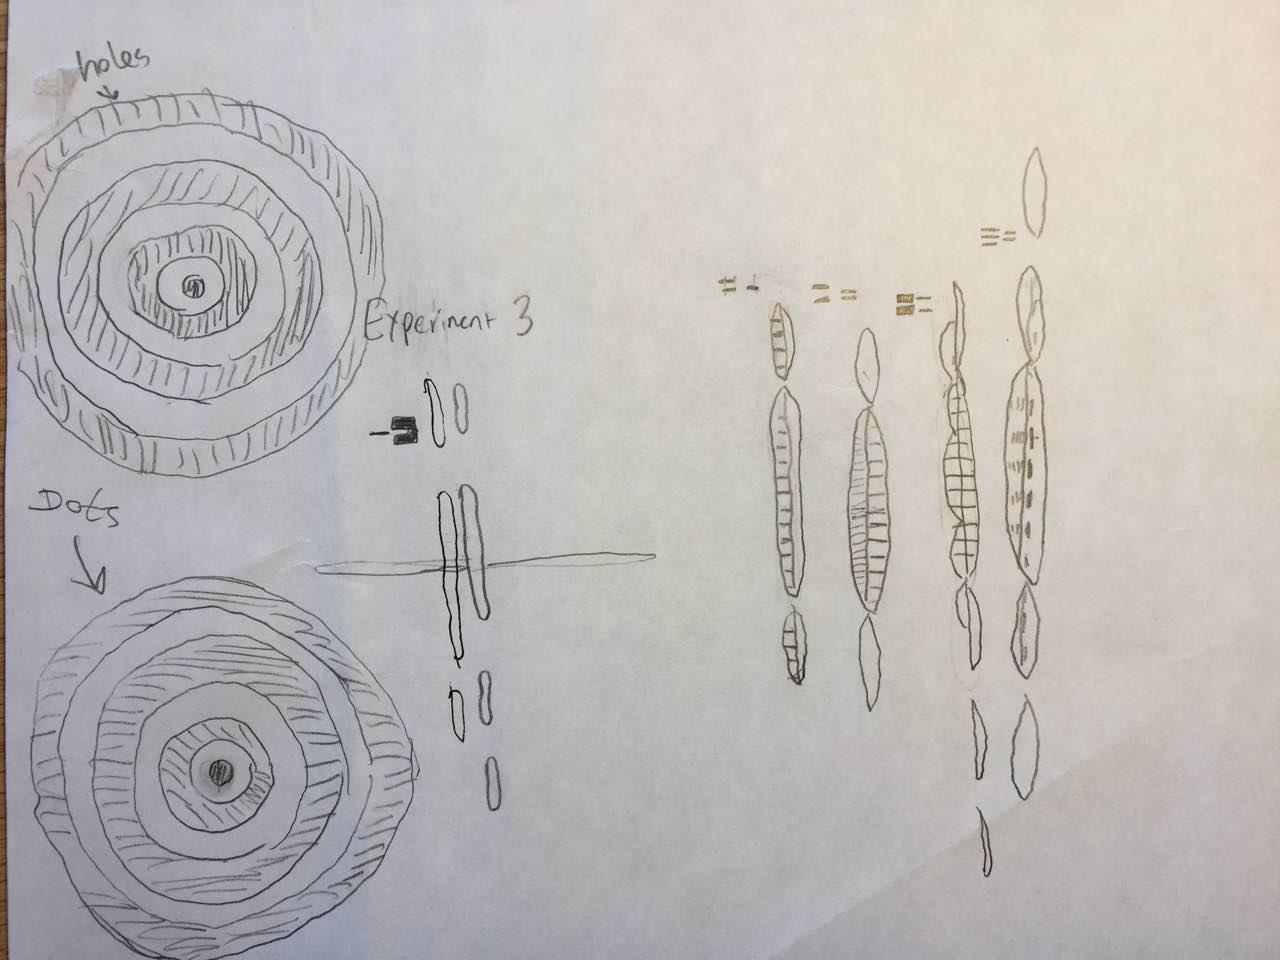
\includegraphics[scale=0.3]{exp3.jpg}
  \end{center}
  \caption{The sketches of the slit disk comparisons and the diffraction
    patterns. The diffraction pattern comparisons are in order from left to
    right.}
\end{figure}

\subsubsection{Questions}

\subsubsubsection{}

\qq While the single and double slits share a wave envelope when the slit width
is the same, the single slit lacks the smaller division within the envelope
present in the double slit.

\subsubsubsection{}

\qq As the slit separation is increased, the envelope of the double slit pattern
retains its size, but the separation of the inner minima decreases.

\subsubsubsection{}

\qq As the slit width is increased, the wave envelope bunches together, as seen
in Figure \ref{pic:exp3}, but the inner minima separation stays the same.

\subsubsubsection{}

\qq While the envelope and inner slit separation is the same between double and
triple slit patterns, the triple slit pattern has another diffraction pattern
occurring each maximum that is perpendicular to the inner pattern of the double
slit.

\subsubsubsection{}

\qq While the diffraction patterns from both a slit and a line share envelope
patterns, they have some noteworthy differences. Not only does the line allow
far more light to pass through than the slit, it also has a horizontal component
to its pattern that the slit lacks.

\subsubsubsection{}

\qq While both the dot pattern and hole patterns form concentric rings, the dot
pattern is darker than the hole pattern, but it has more well defined rings. 

%-----------END EXPERIMENT 3-----------

%----------BEGIN CONCLUSION----------

\section{Conclusion}

\qq Experiment 1 was a success because the percent difference between the
calculated and theoretical slit widths was relatively small; the greatest
difference is for the second order calculations at
\(7.52 \pm \num{78.3e-3} \%\). Experiment 2 was similarly successful, with a
maximum percent difference of only \(2.76 \pm \num{390e-3} \%\). The differences
between the several comparisons in Experiment 3 were well observed.

%-----------END CONCLUSION-----------

\end{document}
